% Provenance (never printed): old terminale S material on the Earth's internal
% heat (geothermal gradient and heat flow, radioactive heat production,
% conduction and convection, mantle convection, geothermal energy). Owner
% (Sync 0/1): heat flow, radiogenic heat production, secular cooling, thermal
% and mantle convection (recall the convection cell of Book 1 g8 first),
% geothermal energy. Geotherm and geothermal gradient are g11.03's; radioactivity,
% half-life, decay law and thermal conductivity are physics' (thermal
% conductivity used as "the rock's thermal conductivity k", never defined);
% hotspot track and plume g11.04's. Figures: figdata/grade-12/internal_heat.py.
\chapter{الحرارة الداخلية للأرض}\label{ch:g12:internal-heat}

بين عامَي 1987 و1995، قرب قرية فينديشيشنباخ في بافاريا، حفر
الجيولوجيون بئرًا عمقها \qty{9101}{m} في \omterm{def:g12:continental-crust:continental-crust}{القشرة القارية}. وفي
القاع كانت حرارة الصخر نحو \qty{265}{\celsius}، وهي أشد من أن يُحفر
أعمق من ذلك.
% ledger: gfz:ktb, gfz:ktb30

الارتفاع من نحو \qty{10}{\celsius} عند السطح إلى \qty{265}{\celsius} على عمق
\qty{9.1}{km} زيادة بنحو \qty{28}{\celsius} لكل كيلومتر، وهي قيمة
نموذجية. ففي كل مكان من الأرض تزداد الحرارة نحو الأسفل، ولذلك تتدفق الحرارة خارجة من
الأرض في كل حين. يقيس هذا الفصل ذلك التدفق، ويسأل من أين تأتي الحرارة،
ويبيّن كيف تنتقل.
% values: ktb_gradient 28.0 (internal_heat.py, surface temperature taken as 10 degC); ledger: gfz:ktb (gradient about 28 K/km)

\begin{recall}
\omterm{def:g11:lithosphere-asthenosphere:geotherm}{المنحنى الحراري الأرضي} هو منحنى درجة الحرارة بدلالة العمق تحت مكان ما،
\omterm{def:g11:lithosphere-asthenosphere:geotherm}{والتدرج الحراري الأرضي} هو ارتفاع درجة الحرارة لكل كيلومتر؛ وتقيس الآبار
من 25 إلى \qty{30}{\celsius} لكل كيلومتر قرب السطح
(\cref{ch:g11:lithosphere-asthenosphere}). وبعض الذرات مشعة: فهي
تتفكك عشوائيًا، ويتناقص عدد الباقي منها إلى النصف كل عمر نصف، وكل
تفكك يحرر طاقة تنتهي حرارةً (كتب الفيزياء). وخلية
الحمل حلقة من مائع يُسخَّن من الأسفل، فيصعد وينتشر
ويبرد ويغوص (الكتاب 1، الصف 8). وعند البقعة الساخنة، تتحرك صفيحة فوق عمود صاعد
من الوشاح الساخن (\cref{ch:g11:plate-motions}).
\end{recall}
% ledger: usgs:gradient-29 (Book 1 row)

\section{التدرج والتدفق الحراري}

\begin{definition}[التدفق الحراري]\label{def:g12:internal-heat:heat-flow}
\emph{التدفق الحراري}\index{تدفق حراري} (أو الدفق الحراري) في مكان ما هو
القدرة التي تغادر باطن الأرض عبر كل متر مربع من سطحها
هناك. ويُقاس بالملّيواط لكل متر مربع
(\unit{mW/m^2}).
\end{definition}
% ledger: b2dd10:continents

تنتقل الحرارة من الساخن إلى البارد، وكلما اشتد تدرج درجة الحرارة،
أسرع انتقالها. ويتوقف مقدار ما ينتقل أيضًا على الصخر: فلكل صخر
موصلية حرارية $k$، بالواط لكل متر لكل كلفن، تعرّفها كتب
الفيزياء.

\begin{proposition}[التدفق الحراري والتدرج]\label{prop:g12:internal-heat:fourier}
عبر صخر موصليته الحرارية $k$ ترتفع فيه درجة الحرارة مع
العمق بتدرج $G$ (بالكلفن لكل متر)، يكون \omterm{def:g12:internal-heat:heat-flow}{التدفق الحراري} الصاعد نحو
السطح
\[
  q = k\,G .
\]
\end{proposition}

هذا القانون للتوصيل، المنسوب إلى فورييه، مسلَّم به هنا؛ وتبرهنه كتب الفيزياء
في صورة عامة.

\begin{method}[التدفق الحراري من بئر]\label{met:g12:internal-heat:borehole}
\begin{enumerate}
  \item قِس درجة الحرارة على عدة أعماق من بئر، بعد أن يكون
        البئر قد أخذ وقته ليعود إلى درجة حرارة الصخر.
  \item ارسم درجة الحرارة بدلالة العمق وخذ الميل: فهو التدرج $G$،
        محوَّلًا إلى كلفن لكل متر.
  \item قِس الموصلية $k$ للصخر على عينات لبية في
        المختبر.
  \item اضرب: $q = kG$، بوحدة \unit{W/m^2}، ثم حوّل إلى \unit{mW/m^2}.
\end{enumerate}
\end{method}

\begin{example}[بئر في الغرانيت]\label{ex:g12:internal-heat:borehole}
بئر في غرانيت موصليته \qty{2.72}{W/(m.K)} يقيس
تدرجًا قدره \qty{29}{\celsius} لكل كيلومتر، أي \qty{0.029}{K/m}.
إذن $q = 2.72 \times 0.029 \approx \qty{0.079}{W/m^2}$، أي نحو
\qty{79}{mW/m^2}.
\end{example}
% ledger: roy:conductivity (granitic layer 6.5 mcal/(cm s degC) = 2.72 W/m/K), usgs:gradient-29 (Book 1 row)
% values: borehole_q_mW 78.9 (internal_heat.py)

جُمع أكثر من \num{38000} قياس من هذا النوع في خريطة
للأرض كلها. تفقد القارات في المتوسط \qty{70.9}{mW/m^2}، وقاع المحيط
\qty{105.4}{mW/m^2}؛ وعلى السطح كله، \qty{91.6}{mW/m^2}.
وبالضرب في مساحة الأرض، \qty{5.101e14}{m^2}، يكون المجموع
\[
  0.0916 \times \num{5.101e14} \approx \qty{4.67e13}{W} = \qty{46.7}{TW},
\]
أي نحو 47 تيراواط، بزيادة أو نقصان 2.
% ledger: b2dd10:continents, b2dd10:half-space (47 +- 2 TW, 38,347 measurements)

يفقد قاع المحيط أكثر ما يفقد حيث يكون أحدث عمرًا. \omterm{def:g11:lithosphere-asthenosphere:lithosphere}{فالغلاف الصخري} الجديد يغادر
الظهرة ساخنًا، ويبرد كلما ابتعد؛ ويتناقص تدفقه الحراري تناسبًا عكسيًا مع
الجذر التربيعي لعمره.

\begin{omfigure}
\begin{tikzpicture}
\begin{axis}[omrecord, width=0.72\linewidth, height=5.6cm, xmin=0, xmax=180, ymin=0, ymax=400,
  xlabel={\foreignlanguage{arabic}{عمر قاع المحيط بملايين السنين}}, ylabel={\foreignlanguage{arabic}{التدفق الحراري \babelsublr{(\unit{mW/m^2})}}},
  xtick={0,30,...,180}, ytick={0,100,...,400}]
% computed in figdata/grade-12/internal_heat.py; ledger: b2dd10:half-space, b2dd10:continents
\addplot[omDef, line width=1.1pt, restrict x to domain=0:66.5] table[x=t_Myr, y=q] {figdata/out/grade-12-internal_heat-halfspace.dat};
\addplot[omDef, line width=1.1pt, densely dotted, restrict x to domain=66.5:180] table[x=t_Myr, y=q] {figdata/out/grade-12-internal_heat-halfspace.dat};
\addplot[omProp, line width=0.9pt, dashed, domain=0:180] {70.9};
\coordinate (lawlab) at (axis cs:14,250);
\coordinate (contlab) at (axis cs:100,80);
\end{axis}
\node[font=\scriptsize, text=omDef, anchor=west] at (lawlab) {$q = 490/\sqrt{t}$};
\node[font=\scriptsize, text=omProp, anchor=south west] at (contlab) {\foreignlanguage{arabic}{متوسط القارات، \babelsublr{\qty{70.9}{mW/m^2}}}};
\end{tikzpicture}

{\small \omterm{def:g12:internal-heat:heat-flow}{التدفق الحراري} عبر قاع المحيط بدلالة عمره، كما حُسب من
تبرد \omterm{def:g11:lithosphere-asthenosphere:lithosphere}{الغلاف الصخري} ($t$ بملايين السنين)؛ وبعد 66.5
مليون سنة (الخط المنقط) يُعرف أن القانون أقل مطابقة. المصدر: ديفيز
وديفيز (2010).}
\end{omfigure}
% values: q_1Myr 490, q_10Myr 155, q_66.5Myr 60.1, age_where_q_equals_cont_Myr 47.8 (internal_heat.py)

\section{من أين تأتي الحرارة}

للحرارة مصدران. أولهما النشاط الإشعاعي.

\begin{definition}[إنتاج الحرارة الإشعاعية]\label{def:g12:internal-heat:heat-production}
\emph{إنتاج الحرارة الإشعاعية}\index{إنتاج الحرارة الإشعاعية} في
صخر ما هو الحرارة المتحررة داخله من تفكك ذراته المشعة،
لكل وحدة حجم ولكل وحدة زمن، بالميكروواط لكل متر مكعب
(\unit{\micro W/m^3}). ويأتي كله تقريبًا من أربعة نظائر: اليورانيوم-238،
واليورانيوم-235، والثوريوم-232، والبوتاسيوم-40.
\end{definition}
% ledger: dye12:isotopes, earle:heat-sources, kamland11:geonu

تتركز هذه العناصر في صخور \omterm{def:g12:continental-crust:continental-crust}{القشرة القارية}. فمن
2188 تحليلًا، يبلغ الوسيط لإنتاج الحرارة في الغرانيت
\qty{2.43}{\micro W/m^3}، وفي البازلت \qty{0.21}{\micro W/m^3}، وفي
الصخور فوق المافية للوشاح \qty{0.11}{\micro W/m^3} فقط، أي أقل بنحو عشرين
مرة من الغرانيت. وطبقة غرانيت سمكها \qty{10}{km} تنتج
$2.43 \times 10^{-6} \times \num{10000} \approx \qty{0.024}{W}$ تحت كل
متر مربع، أي \qty{24}{mW/m^2}: ثلث \omterm{def:g12:internal-heat:heat-flow}{التدفق الحراري} للقارات.
% ledger: b2vila:heat-production, b2dd10:continents
% values: granite_10km_mW 24.3, granite_over_ultramafic 21.9 (internal_heat.py)

كم من الحرارة يصنع النشاط الإشعاعي في الأرض كلها؟ يلتقط كاملاند، وهو
كاشف تحت الأرض في اليابان يحوي 1000 طن من سائل،
النيوترينوات الأرضية، وهي النيوترينوات المضادة التي يحررها تفكك اليورانيوم والثوريوم
داخل الأرض: وقد رصد أولها في 2005، وفي 2135 يومًا من
التسجيل، رصد نحو 106 منها بين 841 حدثًا مرشحًا. ومن ذلك العدد،
مع أعداد كاشف في إيطاليا، يتبين أن اليورانيوم-238 والثوريوم-232 معًا
يحرران نحو 20 تيراواط. أما البوتاسيوم-40 فيفلت من الكاشف؛ ومعلوم
أنه يضيف نحو \qty{4}{TW}، واليورانيوم-235، محسوبًا بالتناسب مع اليورانيوم-238، نحو
\qty{0.4}{TW}. فالنشاط الإشعاعي يوفر إذن نحو \qty{24}{TW}،
أي قرابة نصف \qty{47}{TW} التي تفقدها الأرض.
% ledger: kamland11:geonu, dye12:isotopes, b2dd10:continents
% values: now_K40_TW 4.0, now_U235_TW 0.42, radiogenic_TW 24.4, share_radiogenic 0.523 (internal_heat.py)

\begin{definition}[التبرد القرني]\label{def:g12:internal-heat:secular-cooling}
\emph{التبرد القرني}\index{تبرد قرني} للأرض هو فقدانها البطيء
للحرارة المختزنة فيها منذ تكوّنها، وهي الحرارة الأولية: أي
جزء \omterm{def:g12:internal-heat:heat-flow}{التدفق الحراري} الذي لا يعوّضه النشاط الإشعاعي، والذي به يبرد
الوشاح واللب على مر العصور.
\end{definition}
% ledger: kamland11:geonu, earle:heat-sources

\begin{omfigure}
\begin{tikzpicture}
\begin{axis}[omrecord, xbar stacked, bar width=14pt, width=0.66\linewidth, height=3.2cm, scale only axis,
  xmin=0, xmax=50, ymin=0.4, ymax=2.6, ytick={1,2}, yticklabels={{المصادر}, {الخسائر}},
  xlabel={\foreignlanguage{arabic}{القدرة \babelsublr{(\unit{TW})}}}, ymajorgrids=false, legend columns=2, legend cell align=left,
  legend style={font=\scriptsize, at={(0.5,-0.42)}, anchor=north, /tikz/every even column/.append style={column sep=6pt}}]
% computed in figdata/grade-12/internal_heat.py; ledger: kamland11:geonu, dye12:isotopes, b2dd10:continents
\addplot[fill=omThm!55, draw=omThm] table[x=uth, y=bar] {figdata/out/grade-12-internal_heat-budget.dat};
\addplot[fill=omThm!25, draw=omThm] table[x=kuf, y=bar] {figdata/out/grade-12-internal_heat-budget.dat};
\addplot[fill=omDef!35, draw=omDef] table[x=secular, y=bar] {figdata/out/grade-12-internal_heat-budget.dat};
\addplot[fill=black!25, draw=black!60] table[x=surface, y=bar] {figdata/out/grade-12-internal_heat-budget.dat};
\legend{{اليورانيوم-238 والثوريوم-232، من النيوترينوات الأرضية}, {البوتاسيوم-40 واليورانيوم-235}, {التبرد القرني، أي الباقي}, {التدفق الحراري عند السطح}}
\end{axis}
\end{tikzpicture}

{\small ميزانية الأرض الحرارية اليوم: ما يغادر السطح (العمود العلوي)
وما يوفره (العمود السفلي). المصادر: كاملاند (2011)؛ ديفيز وديفيز
(2010)؛ داي (2012).}
\end{omfigure}
% values: radiogenic_TW 24.4, secular_TW 22.3 (internal_heat.py)

كان النشاط الإشعاعي أقوى في الماضي. فكل نظير يتفكك، فكان
منه في الماضي البعيد أكثر: قبل عمر نصف واحد، ضعف الكمية، وضعف
الحرارة. والرجوع $t$ سنة إلى الوراء يضرب حرارة نظير عمر نصفه
$T$ في $2^{t/T}$.

\begin{proposition}[الحرارة الإشعاعية في الماضي]\label{prop:g12:internal-heat:past}
إذا كان نظير عمر نصفه $T$ يحرر اليوم قدرة $H_0$، فقد حرر
\[
  H(t) = H_0 \, 2^{t/T} = H_0\, e^{\lambda t}, \qquad \lambda = \frac{\ln 2}{T},
\]
قبل زمن $t$.
\end{proposition}

\begin{proof}
القدرة متناسبة مع العدد $N$ من الذرات الباقية، لأن كل
ذرة تتفكك بالاحتمال نفسه في الثانية. وبحسب قانون التفكك، ينقسم $N$
على 2 كل عمر نصف: $N_{\text{الآن}} = N(t)\,2^{-t/T}$، إذن $N(t) =
N_{\text{الآن}}\,2^{t/T}$، ومنه تأتي القدرة. وأخيرًا $2^{t/T} =
e^{(t/T)\ln 2} = e^{\lambda t}$.
\end{proof}

\begin{omfigure}
\begin{tikzpicture}
\begin{axis}[omrecord, width=0.72\linewidth, height=6cm, xmin=0, xmax=4.5, ymin=0, ymax=120,
  x dir=reverse, xlabel={\foreignlanguage{arabic}{الزمن قبل الحاضر بمليارات السنين}}, ylabel={\foreignlanguage{arabic}{الحرارة الإشعاعية \babelsublr{(\unit{TW})}}},
  xtick={0,0.5,...,4.5}, ytick={0,20,...,120}, x tick label style={/pgf/number format/.cd, fixed, precision=1},
  legend pos=north east, legend style={font=\scriptsize}, legend cell align=left]
% computed in figdata/grade-12/internal_heat.py; ledger: kamland11:geonu, dye12:isotopes, nndc:halflives
\addplot[black, line width=1.2pt] table[x=t_Ga, y=total] {figdata/out/grade-12-internal_heat-past.dat};
\addplot[omThm, line width=0.9pt] table[x=t_Ga, y=U235] {figdata/out/grade-12-internal_heat-past.dat};
\addplot[omProp, line width=0.9pt, densely dashed] table[x=t_Ga, y=K40] {figdata/out/grade-12-internal_heat-past.dat};
\addplot[omDef, line width=0.9pt] table[x=t_Ga, y=U238] {figdata/out/grade-12-internal_heat-past.dat};
\addplot[omMeth, line width=0.9pt, densely dotted] table[x=t_Ga, y=Th232] {figdata/out/grade-12-internal_heat-past.dat};
\legend{المجموع, اليورانيوم-235, البوتاسيوم-40, اليورانيوم-238, الثوريوم-232}
\end{axis}
\end{tikzpicture}

{\small الحرارة التي حررتها النظائر المشعة الأربعة رجوعًا إلى
تكوّن الأرض، محسوبة من قيم اليوم بقانون التفكك. أعمار النصف:
الثوريوم-232، 14.0 مليار سنة؛ واليورانيوم-238، 4.468؛ والبوتاسيوم-40، 1.248؛
واليورانيوم-235، 0.704.}
\end{omfigure}
% values: total_4.5Ga_TW 115.9, ratio_total_4.5Ga 4.75, ratio_U235_4.5Ga 84.0, ratio_K40_4.5Ga 12.2, share_U235_K40_4.5Ga 0.72 (internal_heat.py)

قبل أربعة مليارات ونصف مليار سنة، كان النشاط الإشعاعي يحرر نحو
\qty{116}{TW}، أي قرابة خمسة أضعاف قيمة اليوم، وكان معظمها يأتي من
اليورانيوم-235 والبوتاسيوم-40، النظيرين القصيرَي العمر، اللذين كادا
يختفيان منذ ذلك الحين. فقد كان باطن الأرض الفتية أسخن بكثير مما هو اليوم.
% ledger: earle:heat-sources (radiogenic heat now roughly 25 % of what it was)

\section{التوصيل والحمل الحراري}

لا تعبر الحرارة الجسم الصلب إلا بالتوصيل، من ذرة إلى ذرة، وهذا في الصخر
بطيء جدًا. فالحرارة تعبر مسافة $L$ بالتوصيل في زمن
يقارب $L^2/\kappa$، حيث $\kappa$، الانتشارية الحرارية للصخر،
نحو \qty{1e-6}{m^2/s}. وللوشاح الذي سمكه
\qty{2891}{km}،
\[
  \frac{(\num{2.891e6})^2}{\num{1e-6}} \approx \qty{8.4e18}{s} \approx
  \num{2.6e11} \text{ سنة},
\]
أي نحو 260 مليار سنة، قرابة ستين ضعف عمر الأرض. ولو كان الوشاح
لا ينقل الحرارة إلا بالتوصيل، لظلت حرارة أعماقه كلها تقريبًا باقية فيها.
% ledger: england:kelvin (Book 3 row: kappa 1e-6 m2/s), data:prem (CMB at 2891 km)
% values: conduction_time_Gyr 264.9 (internal_heat.py)

الوشاح صلب، لكنه على مدى ملايين السنين يزحف، ببطء شديد، كما
يفعل مائع شديد اللزوجة: \omterm{def:g11:lithosphere-asthenosphere:lithosphere}{فالغلاف اللدن} ينساب (\cref{ch:g11:lithosphere-asthenosphere}).
ولذلك يفقد الوشاح حرارته كما يفعل الهواء فوق المدفأة، بحملها معه.

\begin{definition}[الحمل الحراري؛ الحمل الحراري في الوشاح]\label{def:g12:internal-heat:convection}
\emph{الحمل الحراري}\index{حمل حراري} هو نقل الحرارة
بحركة المادة نفسها: فالمادة الأدفأ والأخف تصعد،
والمادة الأبرد والأكثف تغوص، كما في خلية الحمل.
و\emph{الحمل الحراري في الوشاح}\index{حمل حراري في الوشاح} هو الحمل
الحراري لوشاح الأرض الصلب، الذي يزحف ببضعة سنتيمترات في
السنة وينقل حرارة الباطن نحو السطح.
\end{definition}
% ledger: earle:heat-sources (solid mantle flows at centimetres a year)

الصفائح هي الجزء العلوي من هذا الحمل. فعند الظهرات يصعد الوشاح الساخن
ويُضاف إلى الصفائح؛ ويبرد \omterm{def:g11:lithosphere-asthenosphere:lithosphere}{الغلاف الصخري} كلما ابتعد،
فتزداد كثافته، ويغوص تحت ثقله في نطاقات \omterm{def:g11:subduction-zones:subduction}{الاندساس}: \omterm{def:g11:subduction-zones:slab}{فالألواح المندسة}
هي الجزء البارد الغائص من الجريان، وتُظهرها الصور الزلزالية
غائصة عميقًا في الوشاح. ويُعتقد أن أعمدة من الصخر الساخن تصعد تحت
البقع الساخنة من أعماق الوشاح، وربما من فوق اللب مباشرة.
% ledger: dye12:bse, earle:plume

\begin{omfigure}
\begin{tikzpicture}[x=1cm, y=1cm, font=\scriptsize]
  % mantle annulus sector
  \fill[omLithPeridotite!40] (0,0) ++(20:6.4) arc (20:160:6.4) -- ++(160:-3.2) arc (160:20:3.2) -- cycle;
  \fill[black!45] (0,0) ++(20:3.2) arc (20:160:3.2) -- (0,0) -- cycle;
  \node[white] at (0,1.6) {اللب};
  % lithosphere
  \fill[black!15, draw=black!50] (0,0) ++(20:6.4) arc (20:160:6.4) -- ++(160:-0.3) arc (160:20:6.1) -- cycle;
  % ridge (top) and two trenches
  \draw[omThm, line width=1pt, -{Stealth}] (0,5.9) -- (0,6.35);
  \node[anchor=south] at (0,6.45) {ظهرة};
  \foreach \a/\lab in {48/خندق, 132/خندق} {
    \node[anchor=south] at (\a:6.5) {\lab};
  }
  % slabs (cold, blue) sinking from the trenches
  \draw[omDef, line width=3pt] (48:6.2) .. controls (52:5.2) and (60:4.4) .. (62:3.4);
  \draw[omDef, line width=3pt] (132:6.2) .. controls (128:5.2) and (120:4.4) .. (118:3.4);
  % plume (hot, red) rising
  \draw[omThm, line width=2.4pt] (155:3.25) .. controls (154:4.2) and (152:5.2) .. (151:6.05);
  \fill[omThm] (151:6.0) circle (0.18);
  \node[anchor=west, text=omThm] at (145:4.0) {\foreignlanguage{arabic}{عمود صاعد؟}};
  % convection arrows
  \draw[-{Stealth}, black!65, line width=0.8pt] (80:5.7) arc (80:58:5.7);
  \draw[-{Stealth}, black!65, line width=0.8pt] (100:5.7) arc (100:122:5.7);
  \draw[-{Stealth}, black!65, line width=0.8pt] (68:3.7) .. controls (80:3.6) and (88:4.5) .. (90:5.4);
  \draw[-{Stealth}, black!65, line width=0.8pt] (112:3.7) .. controls (100:3.6) and (92:4.5) .. (90:5.4);
  \node[omDef, anchor=north west, align=left] at (52:4.55) {لوح مندس بارد\\يغوص};
  \node[anchor=north, white] at (90:2.95) {الحد بين اللب والوشاح};
  \node[anchor=south east] at (150:6.45) {الصفائح};
\end{tikzpicture}

{\small \omterm{def:g12:internal-heat:convection}{الحمل الحراري في الوشاح} (رسم تخطيطي، ليس بمقياس رسم). الصفائح هي
حده العلوي البارد: يصعد الوشاح الساخن تحت الظهرات، وتبرد الصفائح كلما
ابتعدت ثم تغوص عائدة \omterm{def:g11:subduction-zones:slab}{ألواحًا مندسة} عند الخنادق، وبعضها يبلغ الوشاح
السفلي. وقد تصعد أعمدة من الأعماق تحت البقع الساخنة.}
\end{omfigure}
% ledger: dye12:bse, earle:plume

فمعظم الحرارة يغادر الوشاح إذن بالحمل، ولا تُعبر بالتوصيل إلا العشرات الأخيرة
من الكيلومترات، عبر \omterm{def:g11:lithosphere-asthenosphere:lithosphere}{الغلاف الصخري} الصلب ---
وهذا هو التوصيل الذي تقيسه الآبار.
% ledger: dye12:bse (convection the main transport of interior heat), earle:heat-sources

\section{الطاقة الحرارية الأرضية}

\begin{definition}[الطاقة الحرارية الأرضية]\label{def:g12:internal-heat:geothermal}
\emph{الطاقة الحرارية الأرضية}\index{طاقة حرارية أرضية} هي حرارة
باطن الأرض التي يستعملها الناس: ماء ساخن أو بخار من صخر ساخن، يُسحب
عبر آبار للتدفئة أو لتوليد الكهرباء.
\end{definition}
% ledger: eia:geo-use, eia:geo-plants

الحرارة المتدفقة من الأرض ضئيلة حيث تبلغ السطح، نحو
\qty{0.1}{W} تحت كل متر مربع، وهذا أقل بكثير من أن يُستعمل مباشرة. وهي
تصير قابلة للاستعمال حيث تتركز على عمق ضحل. فقرب البراكين،
والصدوع الخسفية والبقع الساخنة، وعلى امتداد حدود الصفائح، يقترب الصخر الساخن من
السطح، ويعود الماء الذي يجري في الصخر المنفذ ساخنًا. وتحتاج محطة
الطاقة إلى ماء شديد الحرارة أو بخار، من نحو 150 إلى
\qty{370}{\celsius}؛ وبعض الحقول تعطي بخارًا جافًا يدير التوربينات
مباشرة. وقد وُلدت أول كهرباء من حرارة الأرض عام 1904 في
لارديريلو، في توسكانا: فأضاءت خمسة مصابيح. وفي أماكن أخرى، يُنقل الماء الساخن من
قرب السطح بالأنابيب إلى المباني لتدفئتها.
% ledger: b2dd10:continents, eia:geo-where, eia:geo-plants (300 to 700 degF), enel:larderello, eia:geo-use

\begin{omfigure}
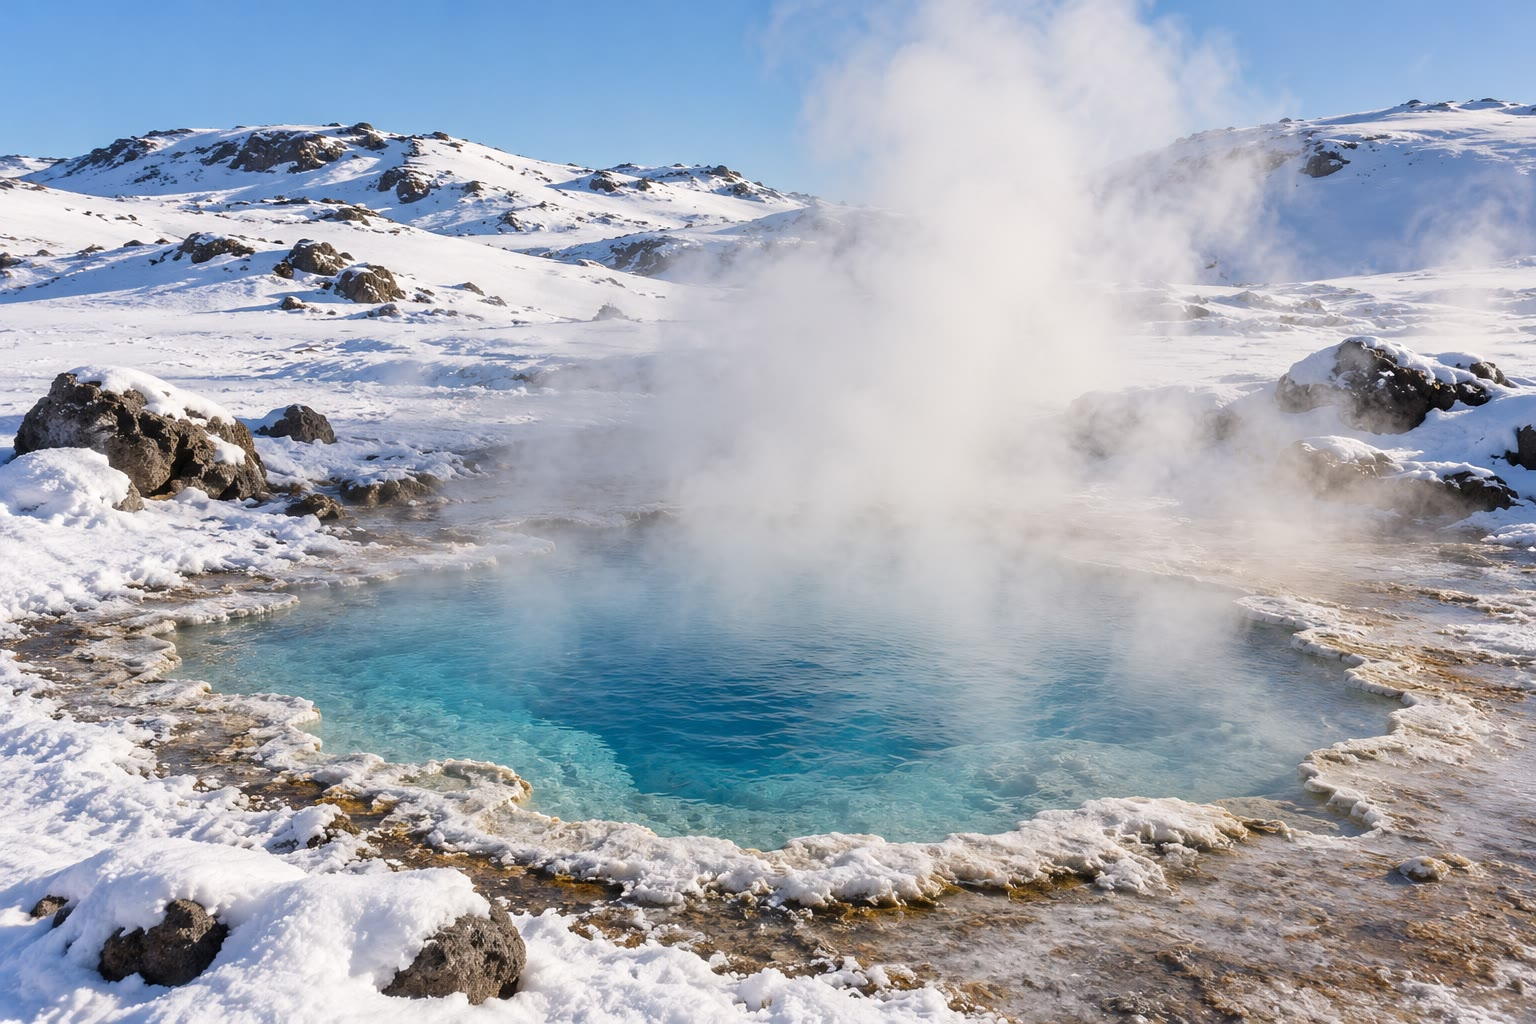
\includegraphics[width=0.6\linewidth]{images/book2/ai/g12-hot-spring-snow.jpg}

{\small ينبوع حار يتصاعد بخاره في منظر ثلجي: ماء سُخّن عميقًا
تحت الأرض يعود إلى السطح. رسم توضيحي مولَّد بالذكاء الاصطناعي.}
\end{omfigure}

\begin{omfigure}
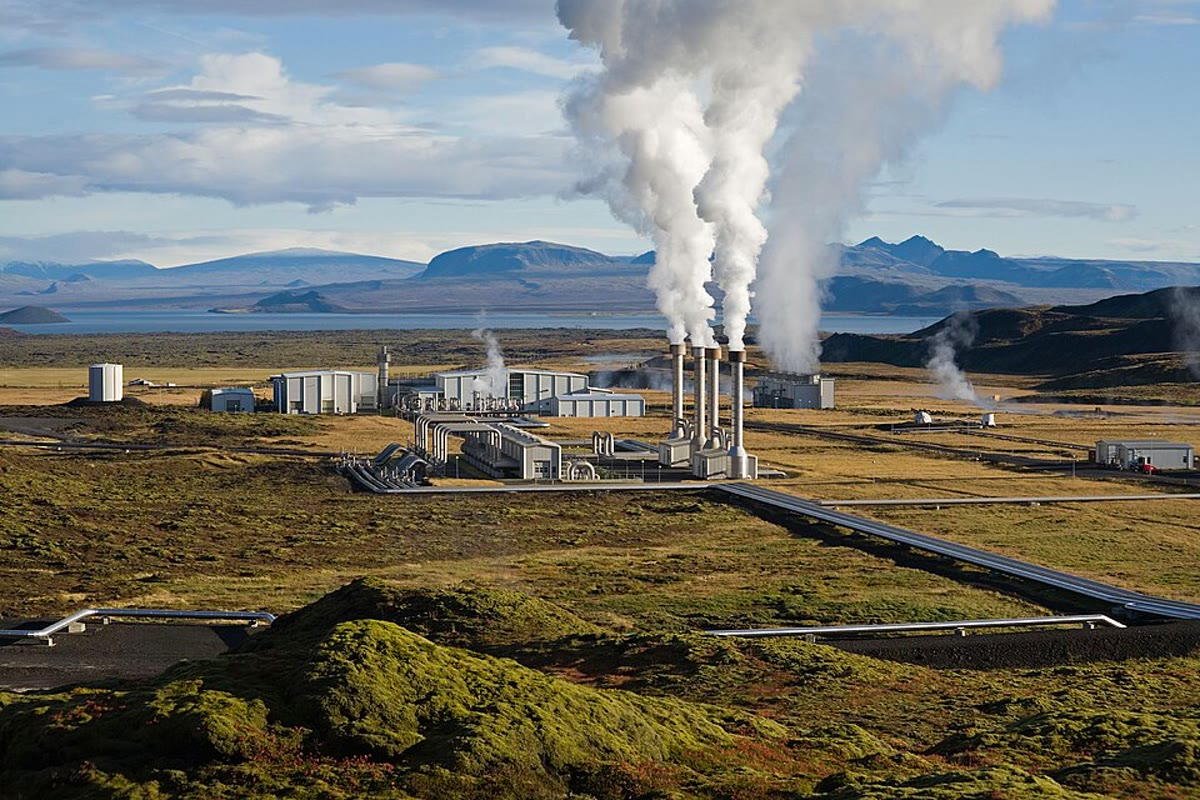
\includegraphics[width=0.66\linewidth]{images/book2/g12-nesjavellir-geothermal.jpg}

{\small محطة نيسيافيتلير \omterm{def:g12:internal-heat:geothermal}{للطاقة الحرارية الأرضية}، في منطقة هينغيل
البركانية في آيسلندا: حتى \qty{120}{MW} من الكهرباء وحتى
\qty{300}{MW} من الحرارة، يحملها الماء الساخن. الصورة: غريتار
إيفارسون (ملك عام).}
\end{omfigure}
% ledger: photo:g12-nesjavellir, on:nesjavellir

الحقل الحراري الأرضي ليس معينًا لا ينضب على مقياس حياة إنسان. ففي
حقل الغايزرز، في كاليفورنيا، سحبت آبار كثيرة جدًا البخار، أسرع مما يستطيع
\omterm{def:g12:internal-heat:heat-flow}{التدفق الحراري} البطيء والمطر تعويضه: فانخفض ضغط البخار
إلى أقل من نصف ذروته، وفُقد أكثر من \qty{40}{\percent} من
قدرة محطات الطاقة. ويُحقن الماء الآن عائدًا إلى
الحقل لإبطاء التراجع.
% ledger: cpuc:geysers

\section{تمارين}

\begin{exercise}[$\star$]\label{exo:g12:internal-heat:1}
أعطِ المصطلح: (أ) القدرة التي تغادر الباطن عبر كل متر مربع
من السطح؛ (ب) الحرارة التي يحررها تفكك الذرات المشعة في وحدة
حجم من الصخر؛ (ج) فقدان الحرارة المختزنة منذ تكوّن الأرض؛
(د) نقل الحرارة بحركة المادة نفسها؛ (ه) حرارة الأرض
الداخلية التي يستعملها الناس.
\end{exercise}

\begin{exercise}[$\star$]\label{exo:g12:internal-heat:2}
حوّل: (1) \qty{91.6}{mW/m^2} إلى \unit{W/m^2}؛ (2) \qty{46.7}{TW} إلى
واط؛ (3) \qty{29}{\celsius} لكل كيلومتر إلى كلفن لكل متر.
\end{exercise}

\begin{exercise}[$\star$]\label{exo:g12:internal-heat:3}
سمِّ النظائر الأربعة التي تصنع الحرارة الإشعاعية كلها تقريبًا، وقل
أي اثنين منها يستطيع كاشف كاملاند رصدهما.
\end{exercise}

\begin{exercise}[$\star$]\label{exo:g12:internal-heat:4}
باستعمال $q = 490/\sqrt{t}$، احسب \omterm{def:g12:internal-heat:heat-flow}{التدفق الحراري} عبر قاع محيط عمره 1 و4
و25 و49 مليون سنة.
\end{exercise}

\begin{exercise}[$\star$]\label{exo:g12:internal-heat:5}
لماذا يُقاس \omterm{def:g12:internal-heat:heat-flow}{التدفق الحراري} في الآبار لا عند السطح نفسه؟
ولماذا يجب الانتظار بعد الحفر قبل القياس؟
\end{exercise}

\begin{exercise}[$\star\star$]\label{exo:g12:internal-heat:6}
في بئر KTB كانت حرارة الصخر نحو \qty{265}{\celsius} على عمق
\qty{9.1}{km}. (1) بأخذ \qty{10}{\celsius} عند السطح، احسب متوسط
التدرج. (2) بموصلية قدرها \qty{2.72}{W/(m.K)}، ما \omterm{def:g12:internal-heat:heat-flow}{التدفق الحراري} الذي
يعطيه؟ (3) قارن بمتوسط القارات.
\end{exercise}

\begin{exercise}[$\star\star$]\label{exo:g12:internal-heat:7}
تغطي القارات \qty{2.073e14}{m^2} بمتوسط \omterm{def:g12:internal-heat:heat-flow}{تدفق حراري} قدره
\qty{70.9}{mW/m^2}، والمحيطات \qty{3.028e14}{m^2} بمتوسط
\qty{105.4}{mW/m^2}. احسب القدرة التي يفقدها كل منهما، والمجموع، وحصة
ما يُفقد عبر قاع المحيط.
\end{exercise}

\begin{exercise}[$\star\star$]\label{exo:g12:internal-heat:8}
طبقة من \omterm{def:g12:subduction-magmatism:granodiorite}{الغرانوديوريت} سمكها \qty{8}{km} إنتاجها الحراري
\qty{1.88}{\micro W/m^3}. (1) ما \omterm{def:g12:internal-heat:heat-flow}{التدفق الحراري} الذي تنتجه عند السطح؟
(2) ما حصته من \qty{70.9}{mW/m^2}؟
\end{exercise}

\begin{exercise}[$\star\star$]\label{exo:g12:internal-heat:9}
عند أي عمر يفقد قاع المحيط من الحرارة قدر ما تفقده القارة المتوسطة،
\qty{70.9}{mW/m^2}، بحسب $q = 490/\sqrt{t}$؟
\end{exercise}

\begin{exercise}[$\star\star$]\label{exo:g12:internal-heat:10}
كم مرة كانت الحرارة التي حررها اليورانيوم-235 قبل 1.4 مليار سنة أكبر منها
اليوم؟ والبوتاسيوم-40، قبل 2.5 مليار سنة؟
\end{exercise}

\begin{exercise}[$\star\star$]\label{exo:g12:internal-heat:11}
باستعمال $t \approx L^2/\kappa$ مع $\kappa = \qty{1e-6}{m^2/s}$، كم
تستغرق الحرارة لتعبر بالتوصيل (1) لابة سمكها \qty{10}{m}؛
(2) غلافًا صخريًا سمكه \qty{100}{km}؛ (3) الوشاح؟ عبّر عن كل نتيجة
بوحدات مناسبة.
\end{exercise}

\begin{exercise}[$\star\star\star$]\label{exo:g12:internal-heat:12}
يحرر الثوريوم-232 اليوم نحو \qty{10.4}{TW}، واليورانيوم-238 \qty{9.6}{TW}،
والبوتاسيوم-40 \qty{4.0}{TW}، واليورانيوم-235 \qty{0.42}{TW}. باستعمال
أعمار النصف الواردة في الشكل، احسب حرارة
كل منها قبل 3 مليارات سنة، والمجموع، وحصة النظيرين
القصيرَي العمر.
\end{exercise}

\begin{exercise}[$\star\star\star$]\label{exo:g12:internal-heat:13}
تستطيع محطة نيسيافيتلير أن تقدم حتى \qty{300}{MW} من الحرارة،
يحملها نحو \qty{1640}{L} من الماء الساخن في الثانية. بحرارة نوعية
قدرها \qty{4180}{J/(kg.K)} وكتلة \qty{1}{kg} لكل لتر، بكم
درجة سُخّن هذا الماء؟ وما مساحة القارة المتوسطة التي
تفقد \qty{300}{MW} من الحرارة؟
\end{exercise}

\begin{exercise}[$\star\star\star$]\label{exo:g12:internal-heat:14}
افترض أن صفيحة تستغرق 100 مليون سنة لتنتقل من ظهرة إلى خندق، وأن
حلقة حمل عبر الوشاح كله تستغرق نحو 200 مليون سنة. (1)
قارن هذين الزمنين بالزمن الذي يستغرقه التوصيل عبر الوشاح،
260 مليار سنة. (2) لماذا يستطيع الحمل نقل الحرارة أسرع من ذلك بكثير، مع أن
الوشاح لا يتحرك إلا بضعة سنتيمترات في السنة؟
\end{exercise}

\begin{exercise}[$\star\star\star$]\label{exo:g12:internal-heat:15}
افترض أن اللب يفقد نحو \qty{10}{TW} من الحرارة لصالح الوشاح عبر
\omterm{def:g11:seismic-structure:core}{الحد بين اللب والوشاح}، على عمق \qty{2891}{km}. (1) ما حصة ذلك من
\omterm{def:g12:internal-heat:secular-cooling}{التبرد القرني}، \qty{22.3}{TW}؟ ومن أين يأتي الباقي؟
(2) احسب متوسط \omterm{def:g12:internal-heat:heat-flow}{التدفق الحراري} عبر \omterm{def:g11:seismic-structure:core}{الحد بين
اللب والوشاح}، وقارنه بمتوسط \omterm{def:g12:internal-heat:heat-flow}{التدفق الحراري} عند السطح،
\qty{91.6}{mW/m^2}. (3) لماذا يستطيع اللب الساخن تسخين قاعدة الوشاح
مع أن الوشاح صلب؟
\end{exercise}

\begin{problem}[{مسألة نهاية الأسبوع --- ميزانية الأرض الحرارية}]
\label{pb:g12:internal-heat:1}
% ledger: b2dd10:continents, b2dd10:half-space, kamland11:geonu, dye12:isotopes, dye12:bse, b2vila:heat-production
% values (internal_heat.py): radiogenic 24.4 TW, secular 22.3 TW, share 0.523, K40 4.0, U235 0.42, U238 9.59
قيس \omterm{def:g12:internal-heat:heat-flow}{التدفق الحراري} للأرض في أكثر من \num{38000} موضع.
تفقد القارات في المتوسط \qty{70.9}{mW/m^2} على \qty{2.073e14}{m^2}،
ويفقد قاع المحيط \qty{105.4}{mW/m^2} على \qty{3.028e14}{m^2}.

\medskip
\noindent\textbf{الجزء الأول --- التدفق الحراري والمساحات.}
\begin{enumerate}
  \item تحقق من أن مجموع المساحتين يساوي مساحة كرة نصف قطرها
        \qty{6371}{km}.
  \item ما الكسر الذي يشغله قاع المحيط من السطح؟
  \item لماذا يفقد قاع المحيط من الحرارة لكل متر مربع أكثر مما تفقده
        القارات؟
  \item باستعمال $q = 490/\sqrt{t}$، احسب \omterm{def:g12:internal-heat:heat-flow}{التدفق الحراري} عبر قاع محيط
        عمره 4 ملايين سنة.
  \item يقيس بئر في الغرانيت (\qty{2.72}{W/(m.K)})
        \qty{26}{\celsius} لكل كيلومتر. هل تدفقه الحراري فوق المتوسط
        القاري أم دونه؟
\end{enumerate}

\medskip
\noindent\textbf{الجزء الثاني --- المجموع.}
\begin{enumerate}[resume]
  \item احسب القدرة المفقودة عبر القارات.
  \item احسب القدرة المفقودة عبر قاع المحيط.
  \item اجمعهما: فهذا \omterm{def:g12:internal-heat:heat-flow}{التدفق الحراري} الكلي للأرض، بالتيراواط.
  \item ما متوسط \omterm{def:g12:internal-heat:heat-flow}{التدفق الحراري} على السطح كله؟
  \item لو كان تحت كل قارة \qty{10}{km} من الغرانيت (\qty{24.3}{mW/m^2})،
        فكم تيراواط ينتج؟ قارن بالقدرة المفقودة
        عبر القارات.
\end{enumerate}

\medskip
\noindent\textbf{الجزء الثالث --- الحرارة الإشعاعية.}
\begin{enumerate}[resume]
  \item يعدّ كاملاند النيوترينوات الأرضية الآتية من اليورانيوم-238 والثوريوم-232: وهما معًا
        يحرران نحو \qty{20.0}{TW}، مع \qty{3.9}{kg} من الثوريوم في
        الأرض لكل كيلوغرام من اليورانيوم. ويحرر الكيلوغرام من اليورانيوم
        \qty{94.4}{\micro W} عبر اليورانيوم-238 الذي فيه و\qty{4.10}{\micro W}
        عبر اليورانيوم-235 الذي فيه؛ ويحرر الكيلوغرام من الثوريوم \qty{26.3}{\micro W}.
        احسب حرارة اليورانيوم-238، ثم حرارة اليورانيوم-235.
  \item يضيف البوتاسيوم-40 نحو \qty{4}{TW}. احسب الحرارة الإشعاعية الكلية.
  \item أي نوع من الصخور يحمل معظم هذه العناصر، وأين يوجد؟
  \item هل كانت الحرارة الإشعاعية أكبر أم أصغر قبل 3 مليارات سنة؟ ولماذا؟
\end{enumerate}

\medskip
\noindent\textbf{الجزء الرابع --- التبرد القرني.}
\begin{enumerate}[resume]
  \item ما القدرة التي لا يوفرها النشاط الإشعاعي؟
  \item من أين تأتي؟
  \item احسب حصة \omterm{def:g12:internal-heat:heat-flow}{التدفق الحراري} التي يوفرها \omterm{def:g12:internal-heat:secular-cooling}{التبرد القرني}.
  \item تعطي نماذج تركيب الأرض حرارة إشعاعية من 11 إلى
        \qty{38}{TW}.
        بين أي حصتين يقع الجزء الإشعاعي حينئذ؟
  \item ما الذي ينقل معظم هذه الحرارة عبر الوشاح؟
  \item لخّص: ما الحصة التي يوفرها النشاط الإشعاعي اليوم من الحرارة التي
        تفقدها الأرض؟
\end{enumerate}
\end{problem}
